
\title{Enhancing EDA and Misclassification Analysis through Tree Structure Visualization}
\author{
        Maor Hornstein \\
        \small{Tabular Data Science (89547) - Final Project}\\
}
\date{}

\documentclass[12pt]{article}
\usepackage{graphicx}
\usepackage{caption}
\usepackage{refstyle}

\begin{document}
\maketitle

\begin{abstract}
a short summary of the problem, your solution, and experimental results (up to 200 words).
\end{abstract}

\section{Problem Description}\label{Problem Description}
The focus of the solution is on the Exploratory Data Analysis (EDA) phase, particularly the use of scatter plots in this phase.

Scatter plots are a useful tool in data analysis and visualization due to their simplicity and ability to show the relationship between two or more groups. They are easy to comprehend and interpret, making them accessible for people with diverse backgrounds. Scatter plots help to uncover trends, patterns and outliers, examine the interactions between variables, and to highlight significant aspects of the data

Despite their usefulness, scatter plots have some limitations. For instance, when data points are tightly packed or overlap (often referred to as overplotting), it can be challenging to accurately gauge the actual density of the data. Another significant challenge is distinguishing between groups when they overlap or when there is a small sample size. Lastly, Scatter plot only displays the distribution of the data in two dimensions and does not give insights into density or distribution in additional dimensions.

\section{Solution overview - The ICC plot}\label{Solution overview}
The proposed solution is a tree-based representation offered as an alternative to scatter plots to address their limitations.

The tree structure mimics the process a researcher goes through when analyzing a scatter plot, visually dividing the plane into subplanes and examining the density and distribution of samples in each subplane. \figref{mylabel} bye.

\begin{figure}[h]
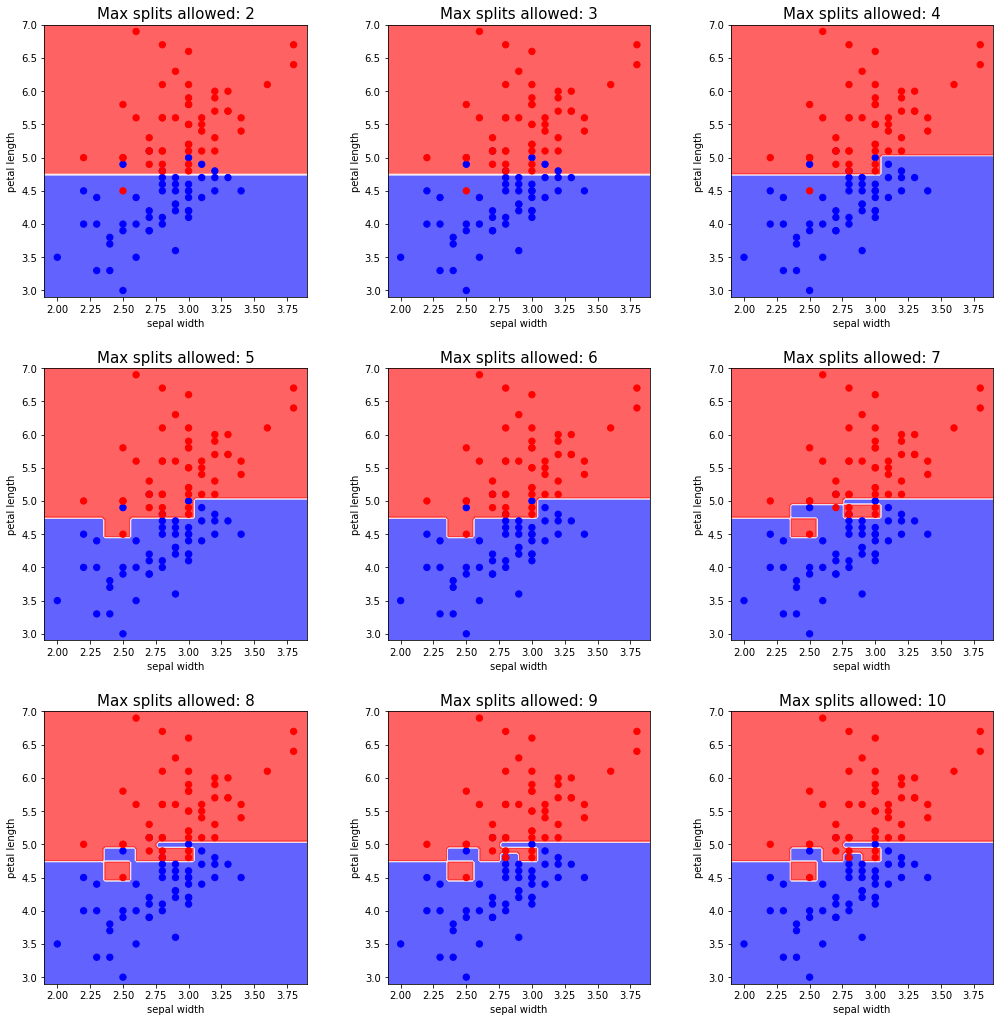
\includegraphics[width=0.8\textwidth]{scatter_plot_illustration.png}
\caption{Illustrates how a researcher visually divides the Scatter plot if he or she uses only horizontal and vertical lines. The simulation is based on a subset of the Iris dataset containing only the Versicolor and Virginica classes and the Sepal width and Petal length attributes.}
\label{fig:mylabel}
\end{figure}


\section{Experimental evaluation}\label{Experimental evaluation}
Explain how you prove that your solution
“works” and provide the details, accompanied with graphs and/or tables.
You must include a comparison table or graph between your solution and
baseline approach(es)

\section{Related work}\label{Related work}
include a short discussion on relevant existing tools and
techniques. *Cite the works as well as discuss them*. Did they try to
solve the same problem? In what manner your solution different? Did
you use/ got inspiration from it? 

\section{Conclusion}\label{Conclusion}
summarize your finding, and the things you learned from
the project

\bibliographystyle{abbrv}
\bibliography{main}

\end{document}